\documentclass[12pt, a4paper]{article}
\usepackage{amsmath}
\usepackage{amsfonts}
\usepackage{amsthm}
\usepackage{mathtools}
\newtheorem{theorem}{Theorem}[section]
\newtheorem{definition}{Definition}[section]
\numberwithin{equation}{section}
\usepackage{pgfplots}
\pgfplotsset{width=10cm,compat=1.9}
\graphicspath{ {img/} }
\DeclareGraphicsExtensions{.png}

\title{Information theory}
\author{Kristian Wichmann}

\begin{document}
\maketitle

\section{Self-information or surprisal}
Let $X$ be a random variable. Consider an event $A$. We may ask ourselves how much information $I(A)$ - also known as \textit{self-information} or \textit{surprisal} - we have gained by having this event occuring. It is clear, that such a quantity must depend only on the probability of the event:
\begin{equation}
I(A)=I(P(A))
\end{equation}
Therefore, we can express self-information through a function $f(p)$, so that if $P(A)=p$, then $I(A)=f(p)$.

If the outcome of an event $A$ is certain, i.e. if $P(A)=1$ then we have gained no information. So we must have $P(A)=1\Rightarrow I(A)=0$. or in other words $f(1)=0$. Non-certain events occuring, on the other hand, should give us non-zero information. So for $p<1$ we should have $f(p)>0$.

Further, if two events $A$ and $B$ are independent it seems reasonable to require that self-information is additive is the following sense:
\begin{equation}
\label{self_information_additivity}
I(A\cap B)=I(A)+I(B)
\end{equation}
So if two independent events happen at the same time, self-information should simply add up. Because of independence, we also have:
\begin{equation}
P(A\cap B)=P(A)\cdot P(B)
\end{equation}
Applying $f$ to both sides of this equation we get:
\begin{equation}
I(A\cap B)=f(P(A)\cdot P(B))
\end{equation}
Combine this with equation $(\ref{self_information_additivity})$ to get:
\begin{equation}
f(P(A)\cdot P(B))=f(P(A))+f(P(B))
\end{equation}
The only functions having this property are logarithms. Hence, the self-information must be of the form:
\begin{equation}
f(p)=-k\cdot\log(p)
\end{equation}
The minus sign comes from requiring $f(p)>0$ for $p<1$. This means that $k$ will be positive, but apart from that can be chosen freely. Since all logarithms are proportional to each other, this is equivalent to choice of base $b$ being free:
\begin{equation}
f(p)=-\log_b(p)
\end{equation}

\subsection{Continous distributions?}
The section above deals with discrete random variables? However, we run into problems if we try to mindlessly generalize to continuous variables: The "obvious" analogue of the self-information for the outcome $X=x$ the would be $-\log_b f(x)$, where $f(x)$ is the probability density function of $X$. But since this function need not be below 1, the associated "surprisal" may actually be negative! Clearly, something is fishy.

\subsubsection{Surprisal for an interval}
The problem is in essence, that a probability density is not a probability. Instead, the probability of finding $X$ realized in an interval of size $\Delta x$ close to $x$ is approximately:
\begin{equation}
P(x\le X<x+\Delta x)\approx f(x)\Delta x
\end{equation}
The surprisal for this event is thus approximately:
\begin{equation}
-\log_b(f(x)\Delta x)=\log_b f(x)-\log_b\Delta x
\end{equation}
In the limit $\Delta x\rightarrow 0$ this should become exact. But here the logarithm tends to minus infinity, and so surprisal is infinite! Which makes sense: Since there's a continuum of outcomes, any specific outcome has probability zero, and hence is infinitely surprising.


\section{Entropy}
The \textit{entropy} of a discrete random variable $X$ is the expectation value of the self-information:
\begin{equation}
H(X)=E[I(X)]=E[-\log_b(X)]
\end{equation}
Here, $I(X)$ is itself a stochastic variable. Thus, entropy can be interpreted as the expected surprisal. Since $X$ is discrete, we may write:
\begin{equation}
\label{entropy_definition}
H(X)=-\sum_x p(x)\log_b p(x)
\end{equation}

Figure \ref{fig:entropy_graph} shows how much an outcome of $p$ contributes to the total entropy. Since the limit for $p\rightarrow 0$ tends to zero, we will extend the definition to outcomes with zero probability; these do not contribute to the entropy.

\begin{figure}
\centering
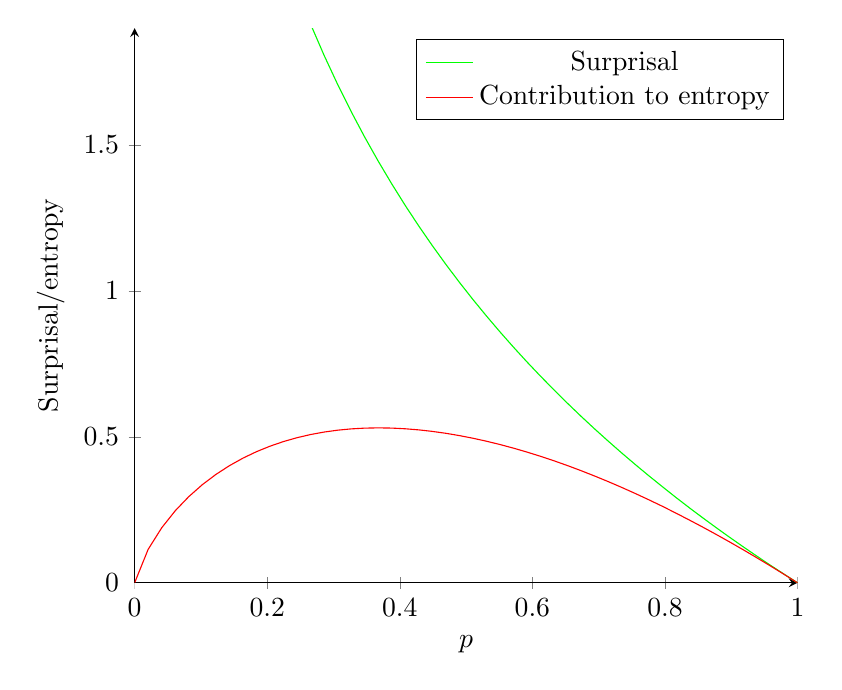
\begin{tikzpicture}
\begin{axis}[
    axis lines = left,
    xlabel = $p$,
    ylabel = {Surprisal/entropy},
    ymin = 0,
    ymax = 1.9,
]
\addplot [
    domain=0:1, 
    samples=50, 
    color=green,
]
{-ln(x)/ln(2)};
\addlegendentry{Surprisal}

\addplot [
    domain=0:1, 
    samples=50, 
    color=red,
]
{-x*ln(x)/ln(2)};
\addlegendentry{Contribution to entropy}
\end{axis}
\end{tikzpicture}
\caption{Surprisal and contribution to entropy as a function of $p$. Here for $b=2$.}
\label{fig:entropy_graph}
\end{figure}

\subsection{Different choices of $b$}
As mentioned above, we're free to choose $b$, but some choices are common. Each carry its own unit of entropy with it:
\begin{itemize}
\item $b=2$: The corresponding entropy is known as \textit{Shannon entropy}, and the unit is Shannon or simply bits.
\item $b=e$: The corresponding unit is known as a nat.
\item $b=10$: The corresponding unit is known as a Hartley.
\end{itemize}
Unless explicitly mentioned, we will use Shannon entropy from now on.

\subsection{Example: Entropy of a coin toss}
Let's consider the simplest possible non-trivial situation: and experiment with two outcomes, $A$ and $B$. If the probability of $A$ is $p$, then the probability of $B$ must be $1-p$.
For a fair coin, both probabilities are $\frac{1}{2}$, and the entropy is:
\begin{equation}
H=-\frac{1}{2}\log_2\frac{1}{2}-\frac{1}{2}\log_2\frac{1}{2}=\frac{1}{2}+\frac{1}{2}=1
\end{equation}
If the coin is not fair, but the probability of tails ($A$) is $p$, instead we get:
\begin{equation}
H(p)=-p\log_2 p-(1-p)\log_2(1-p)
\end{equation}
This function is plotted in figure $\ref{fig:coin_entropy}$.

\begin{figure}
\centering
\begin{tikzpicture}
\begin{axis}[
    axis lines = left,
    xlabel = $p$,
    ylabel = {Surprisal/entropy},
    ymin = 0,
    ymax = 1.1,
]
\addplot [
    domain=0:1, 
    samples=50, 
    color=blue,
]
{-x*ln(x)/ln(2)-(1-x)*ln(1-x)/ln(2)};
\addlegendentry{$H(p)$}
\end{axis}
\end{tikzpicture}
\caption{Entropy for an unfair coin toss.}
\label{fig:coin_entropy}
\end{figure}

\subsection{Entropy of a continuous distribution}
\label{continous_entropy}
As we saw above, the surprisal of any outcome from a continous probability distribution is infinite, but it's not inherently clear whether the entropy should diverge as well. This turns out to actually be true. Writing out the steps in the derivation will actually be useful later. So, let's pick an interval size $\Delta x$ and write an approximate entropy as a sum:
\begin{equation}
H(X)\approx -\sum_{n\in\mathbb{Z}}P(x_n\le X<x_{n+1})\log_2 P(x_n\le X<x_{n+1})
\end{equation}
Here $x_n=n\Delta x$. The probability is approximately $f(x_n)\Delta x$:
\begin{equation}
H(X)\approx -\sum_{n\in\mathbb{Z}}f(x_n)\Delta x\log_2(f(x_n)\Delta x)
\end{equation}
Use the usual formula for the product of a log to split it into two sums:
\begin{equation}
-\underbrace{\sum_{n\in\mathbb{Z}}f(x_n)\log_2(f(x_n))\Delta x}_{\rightarrow\int f(x)\log_2 f(x)\ dx}-\log_2(\Delta x)\underbrace{\sum_{n\in\mathbb{Z}}f(x_n)\Delta x}_{\rightarrow 1}
\end{equation}
The underbraces show what happens when $\Delta x\rightarrow 0$. So, abusing the notation somewhat, the entropy of $X$ is:
\begin{equation}
H(X)=-\int f(x)\log_2 f(x)\ dx-\lim_{\Delta x\rightarrow 0}\log_2\Delta x
\end{equation}
The first term is the \textit{differential entropy}, which is the immediate generalization of equation \ref{entropy_definition}. But we also know that this is not necessarily positive, since probability distributions are not bounded between 0 and 1. This is not absurd, because we need to take the second, infinite term - a \textit{logarithmic divergence} - into account. The differential entropy, as absurd as it may seem, measures the deviation from this infinity is some sense. But the total entropy is infinite.

\subsubsection{Maximum differential entropy}
We might now ask the question: Is there a probability distribution which maximizes differential entropy? Naturally, that the answer to this question depends on our constraints, including the domain/dominating measure of the distribution function. For distributions with all real numbers/Lebesgue measure as dominating measure, with finite mean and variance, the maximum differential entropy distribution is none other than the normal distribution! This is one of the many ways to characterize the Gaussian.

\section{Conditional entropy and mutual information}

\subsection{Entropy of a joint distribution}
Given two discrete random variables $X$ and $Y$, we may define their \textit{joint entropy} simply as the entropy of their joint distribution:
\begin{equation}
H(X,Y)=-\sum_{x,y}P(X=x, Y=y)\log_2\left(P(X=x, Y=y)\right)
\end{equation}
Or using the joint distribution function $p(x,y)=P(X=x, Y=y)$:
\begin{equation}
H(X,Y)=-\sum_{x,y}p(x,y)\log_2 p(x,y)
\end{equation}

\subsection{Conditional entropy}
Similarly, we may define \textit{conditional entropy}. If we already know the outcome of one random variable, this will limit the number of outcomes that contributes to the entropy. But the probabilities become conditional:
\begin{equation}
H(X|Y=y)=-\sum_x p(x|y)\log_2 p(x|y)
\end{equation}
Since $p(x|y)=\frac{p(x,y)}{p(y)}$ this means:
\begin{equation}
\label{conditional1}
H(X|Y=y)=-\sum_x\frac{p(x,y)}{p(y)}\log_2\frac{p(x,y)}{p(y)}
\end{equation}
The total conditional entropy is found by weighing all of these:
\begin{equation}
\label{conditional2}
H(X|Y)=\sum_y p(y)\cdot H(X|Y=y)
\end{equation}
Here $p(y)=\sum_x p(x,y)$ is the marginal probability for $Y$. (Similarly $p(x)=\sum_y p(x,y)$). Inserting equation \ref{conditional1} into equation \ref{conditional2} we get:
\begin{equation}
H(X|Y)=-\sum_y p(y)\sum_x \frac{p(x,y)}{p(y)}\log_2\frac{p(x,y)}{p(y)}=-\sum_{xy}p(x,y)\log_2\frac{p(x,y)}{p(y)}
\end{equation}

\begin{figure}
\centering
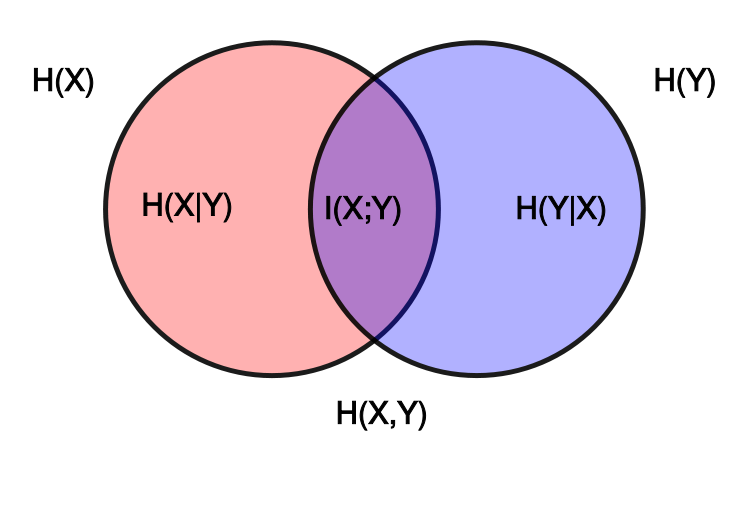
\includegraphics[width=\textwidth]{mutual_information}
\caption{Visualization of the different entropies and mutual information. Image source: Wikipedia.}
\label{fig:mutual_information}
\end{figure}

Looking at figure $\ref{fig:mutual_information}$, we would expect that $H(X,Y)-H(Y)=H(X|Y)$. Let's check that this is indeed the case:
\begin{equation}
H(X,Y)-H(Y)=-\sum_{x,y}p(x,y)\log_2 p(x,y)-\left(-\sum_y p(y)\log_2 p(y)\right)
\end{equation}
Use the definition of $p(y)$:
\begin{equation}
\sum_y p(y)\log_2 p(y)=\sum_{xy}p(x,y)\log_2 p(y)
\end{equation}
Hence:
\begin{equation}
H(X,Y)-H(Y)=-\sum_{x,y}p(x,y)\left(\log_2 p(x,y)-\log_2 p(y)\right)
\end{equation}
This is the same as:
\begin{equation}
-\sum_{x,y}p(x,y)\log_2\frac{p(x,y)}{p(y)}=H(X|Y)
\end{equation}

\subsection{Mutual information}
If we look at figure $\ref{fig:mutual_information}$ once again, we also notice $I(X;Y)$, the \textit{mutual information} between two discrete random variables $X$ and $Y$. It should be equal to:
\begin{equation}
I(X;Y)=H(X)-H(X|Y)
\end{equation}
Inserting we get:
\begin{equation}
-\sum_x p(x)\log_2 p(x)-\left(-\sum_{x,y}p(x,y)\log_2\frac{p(x,y)}{p(y)}\right)
\end{equation}
Now use $p(x)=\sum_y p(x,y)$ to rewrite the first term:
\begin{equation}
\sum_x p(x)\log_2 p(x)=\sum_{xy}p(x,y)\log_2 p(x)
\end{equation}
Combine terms to get:
\begin{equation}
\label{mutual_information}
I(X;Y)=\sum_{x,y}p(x,y)\log_2\frac{p(x,y)}{p(x)p(y)}
\end{equation}
This is clearly symmetrical: $I(X;Y)=I(Y;X)$. Also, if $X$ and $Y$ are independent, then $p(x,y)=p(x)p(y)$ which makes the fraction $1$ and logarithm zero, so the mutual information vanishes in this case.

\subsection{Example: The Monty Hall problem}
In the famous Monty Hall problem, you're presented with three doors, behind which is a prize. After making an initial choice of doors, Monty opens one empty door that you have not chosen, and offers you to change your choice.

As is known, when choosing the first door, all choices are equally likely to get you the prize. If we call this experiment $X$, the entropy is:
\begin{equation}
H(X)=\frac{1}{3}\log_2 3+\frac{1}{3}\log_2 3+\frac{1}{3}\log_2 3=\log_2 3\approx 1.58
\end{equation}

After the door has been opened, however, there's two options with probabilities of $1/3$ and $2/3$ respectively (it's advantageous to change your mind). If we call the event/experiment associated with opening the door $Y$, we might write this as:
\begin{align}
H(X|Y)=&\frac{1}{3}\log_2 3+\frac{2}{3}\log_2\frac{3}{2}=\\
&\frac{1}{3}\log_2 3+\frac{2}{3}(\log_2 3-\log_2 2)=\log_2 3-\frac{2}{3}\approx 0.92
\end{align}

In other words, the mutual information is:
\begin{equation}
I(X;Y)=H(X)-H(X|Y)=\log_2 3-\left(\log_2 3-\frac{2}{3}\right)=\frac{2}{3}
\end{equation}
So the information gain by Monty opening the door is $2/3$ bits.

One might ask how much this is compared to the original uncertainty. This quantity is known as the \textit{percentual information gain} or PIG for short:
\begin{equation}
\textrm{PIG}=\frac{I(X;Y)}{H(X)}=\frac{2/3}{\log_2 3}\approx 42.1\%
\end{equation}
So Monty gives away about $42\%$ of the information away by opening the door. Somewhere, Douglas Adams is smiling \ldots

Now, let's consider the situation from Monty's point of view. He has to choose a door. If he had to choose it without the player having chosen one yet, he would have two option with an equal probability - he cannot open the door with the prize behind it. So the entropy is the same as for a fair coin toss:
\begin{equation}
H(Y)=H=\frac{1}{2}\log_2+\frac{1}{2}\log_2=1
\end{equation}

However, once the player has chosen a door, there's two situations to consider:
\begin{itemize}
\item If the player has indeed chosen the door with the prize behind it, the situation is the same as above:
\begin{equation}
H(Y|X=\textrm{prize})=1
\end{equation}
\item If the player has chosen an empty door, there is only one choice for Monty, namely the other empty door. So the entropy vanished in this case:
\begin{equation}
H(Y|X=\textrm{no prize})=0
\end{equation}
\end{itemize}
We now use equation \ref{conditional2} to get the total conditional entropy:
\begin{equation}
H(Y|X)=\frac{1}{3}\cdot 1+\frac{2}{3}\cdot 0=\frac{1}{3}
\end{equation}
Let's check that we get the same amount of mutual information here:
\begin{equation}
I(X;Y)=H(Y)-H(Y|X)=1-\frac{1}{3}=\frac{2}{3}
\end{equation}
Indeed we do!

Finally, we may ask what Monty's percentual information gain by the player choosing a door is:
\begin{equation}
\textrm{PIG}=\frac{I(X;Y)}{H(Y)}=\frac{2/3}{1}=\frac{2}{3}\approx 66.7\%
\end{equation}

\subsection{Continuous distributions}

\subsubsection{Joint entropy}
Following the same logic as in section \ref{continous_entropy}, we may write the joint entropy is two continuous variables as:
\begin{equation}
H(X,Y)\approx-\sum_{n,m\in\mathbb{Z}}p_{mn}\log_2 p_{mn}
\end{equation}
Here, $p_{nm}=P(x_n\le X<x_{n+1}, y_m\le Y<y_{m+1})$, which is in turn approximately $f(x,y)\Delta x\Delta y$, where $f$ is the joint probability density. Splitting the logarithm, we end up with:
\begin{equation}
H(X,Y)=-\int f(x,y)\log_2 f(x,y)\ dx\ dy-\lim_{\Delta x\rightarrow 0}\log_2\Delta x-\lim_{\Delta y\rightarrow 0}\log_2\Delta y
\end{equation}
Again, this is to be taken with the same grain of salt as before.


\section{Cross-entropy and the Kullback-Leibler divergence}

\subsection{Comparing probability distributions}
Let's say we have two probability distributions $p$ and $q$ for the discrete random variables $X$. The entropy of $X$ will differ according to which distribution we use:
\begin{align}
\label{p_entropy}
H_p(X)=E_p[-\log_2 p(x)]&=-\sum_x p(x)\log_2 p(x)\\
H_q(X)=E_q[-\log_2 q(x)]&=-\sum_x q(x)\log_2 q(x)
\end{align}
Here, we've introduced subscripts on the expectation operator, depending on which distributaion is used. Now, we might use the distribution of $p$ to evalute the $q$-surprise expectation: 
\begin{equation}
\label{crossentropy}
H_{pq}(X)=E_x[-\log_2 p(y)]=-\sum_x p(x)\log_2 q(x)
\end{equation}
This is known as the \textit{cross-entropy}. This is often written as $H(p,q)$, but this alternative notation is used here to to avoid confusion with the joint entropy. Note that in general this is not a symmetric function: $H_{pq}(X)\neq H_{qp}(X)$. Therefore, even is the cross-entropy in some sense measures a difference between the two distributions, it cannot be a metric.

\subsection{Kullback-Leibler divergence}
The \textit{Kullback-Leibler divergence} from $q$ to $p$ (note the appearantly reversed order) is defined as:
\begin{equation}
D_{KL}(p||q)=H_{pq}(X)-H_p(X)
\end{equation} 
Here, the $X$ is understood on the left hand side. Using equations \ref{p_entropy} and \ref{crossentropy} this is:
\begin{equation}
-\sum_x p(x)\log_2 q(x)+\sum_x p(x)\log_2 p(x)=\sum_x p(x)\log_2\frac{p(x)}{q(x)}
\end{equation}
In summary:
\begin{equation}
\label{kl_divergence}
D_{KL}(p||q)=\sum_x p(x)\log_2\frac{p(x)}{q(x)}
\end{equation}
Like cross-entropy, this is asymmetric, so while it still can be used to compare distributions, it is not a metric on distribution space. Hence the name divergence.

\subsection{Connection to mutual information}
Remember that the mutual information (or information gain) between the random variables $X$ and $Y$ is:
\begin{equation}
I(X;Y)=H(X)-H(X|Y)=\sum_{x,y}p(x,y)\log_2\frac{p(x,y)}{p(x)p(y)}
\end{equation}
Here, we've used the formula from equation \ref{mutual_information}. But this is the same as the KL divergence between the distribution functions $p(x,y)$ and $p(x)p(y)$:
\begin{equation}
I(X;Y)=H_{KL}(p(x,y)||p(x)p(y))
\end{equation}
Again we see that mutual information in some sense measures distance to independence.

\section{Model selection}
If we're in a situation where we have a model which outputs a probability distribution $p$ based of the inputs, and we have a target distribution of $y$, then we can use the KL-divergence and cross-entropy as a criterion for selecting a model that is good in some sense.

\subsection{Example: Classification}
A supervised classification problem is a primary example of the situation described above. We have a target distribution given by the one-hot encoding of the label for a given sample: $y_i=\delta_{ij}$, where $j$ is the label. The model will have a number of parameters which we wish to to tune, and the output distribution $p$ depends on these. Based on the last section, a reasonable way to choose parameters, is to require that $y$ deviates as little from $p$ as possible. In other words, we seek to minimize the KL-divergence $D_{KL}(y||p)$. Let's write this out:
\begin{equation}
D_{KL}(y||p)=H_{yp}-H_y
\end{equation}
The entropy of $y$ is simply zero. And more importantly, it's a constant, so it will not matter when minimizing, even if the target distribution was more complex. So model selection has been reduced to choosing the parameters which minimizes the cross-entropy $H_{yp}$. For one sample, this is:
\begin{equation}
-\sum_x y(x)\log_2 p(x)
\end{equation}
Here $x$ runs over the possible cases the classification distinguishes between. When we have $n$ samples, it is customary to use the average cross-entropy:
\begin{equation}
-\frac{1}{n}\sum_{i=1}^n\sum_x y_i(x)\log_2 p_i(x)
\end{equation}
In machine learning, this is known as a \textit{cost function}. This quantity is then minimized, often using some variation of gradient descent.

\end{document}